\documentclass[11pt]{article}

% ---------- Page layout ----------
\usepackage[margin=1in]{geometry}

% ---------- Math ----------
\usepackage{amsmath,amssymb,amsfonts,bm}
\usepackage{mathtools}

% ---------- Graphics / Tables ----------
\usepackage{graphicx}
\usepackage{booktabs}
\usepackage{array}
\usepackage{float}

% ---------- TikZ ----------
\usepackage{tikz}
\usetikzlibrary{arrows.meta,calc,positioning,matrix,patterns,decorations.pathreplacing}

% ---------- Algorithms ----------
\usepackage{algorithm}
\usepackage{algpseudocode}

% ---------- Hyperlinks ----------
\usepackage[colorlinks=true,linkcolor=blue,citecolor=blue]{hyperref}

% ---------- Bibliography ----------
\usepackage[numbers,sort&compress]{natbib}

% ---------- Shortcuts ----------
\newcommand{\Neq}{N_{\rm eq}}
\newcommand{\im}{i_{\rm m}}
\newcommand{\vm}{v_{\rm m}}
\newcommand{\Kii}{\mathcal{K}^{ii}}
\newcommand{\Kvv}{\mathcal{K}^{vv}}
\newcommand{\Kvi}{\mathcal{K}^{vi}}
\newcommand{\Kcav}{\mathcal{K}^{\rm cav}}
\newcommand{\Dsink}{\mathcal{D}}
\newcommand{\eps}{\varepsilon}
\newcommand{\bw}{b}
\newcommand{\rank}{r}
\newcommand{\RR}{\mathbb{R}}
\DeclareMathOperator{\diag}{diag}

\title{Jacobian Structure and Woodbury Preconditioning\\
for the RadCluster Code}
\author{N.\,M.\ Ghoniem}
\date{April 2026}

\begin{document}
\maketitle

\begin{abstract}
The RadCluster cluster dynamics solver integrates a stiff ODE system
of $\Neq = I + V + O(1)$ equations for SIA and vacancy cluster
concentrations. When only monomers are mobile
($\im = \vm = 1$), the Jacobian is a
\emph{bordered tridiagonal} (arrowhead) matrix, and when multiple
mobile species participate in coalescence reactions the Jacobian
becomes a \emph{bordered banded} matrix with a low-rank dense
border. We analyze the sparsity structure in both cases, discuss the
limitations of unpreconditioned and diagonally preconditioned GMRES
for this class of problems, and derive an efficient
\emph{Woodbury preconditioner} that exploits the bordered-banded
decomposition. The preconditioner setup costs
$O(\Neq\,\bw^{2})$ and each solve costs $O(\Neq\,\bw)$, compared
with $O(\Neq^{3})$ for a dense direct solver---a speedup of roughly
$10^{5}$ for typical system sizes.
\end{abstract}

\tableofcontents

%======================================================================
\section{The ODE System}
\label{sec:ode}
%======================================================================

The state vector is
\begin{equation}
  \mathbf{y} = \bigl[\underbrace{c_{1}^{(i)},\ldots,c_{I}^{(i)}}_{I},\;
  \underbrace{c_{1}^{(v)},\ldots,c_{V}^{(v)}}_{V},\;
  Q_{\rm tot},\; c_{h}\bigr]^{T} \in \RR^{\Neq},
  \label{eq:state}
\end{equation}
where $c_{n}^{(i)}$ is the concentration of SIA clusters of size~$n$,
$c_{m}^{(v)}$ the marginal vacancy/bubble concentration of
size~$m$, $Q_{\rm tot}$ the total He content, and $c_{h}$ the free He
monomer concentration (omitted when quasi-steady-state He is used).

The master equations (ME$_{\rm SIA}$, ME$_{\rm vac}$, ME$_{\rm He}$) from
the RadCluster formulation~\cite{Ghoniem2026} couple the state
variables through the following reactions:

\begin{enumerate}
  \item \textbf{SIA--SIA coalescence:}
    $I_{n'} + I_{n-n'} \to I_{n}$ for mobile $n' \le \im$.
  \item \textbf{V--V coalescence:}
    $V_{m'} + V_{m-m'} \to V_{m}$ for mobile $m' \le \vm$.
  \item \textbf{V--I annihilation:}
    $V_{m'} + I_{n} \to I_{n-m'}$ for mobile $m' \le \vm$.
  \item \textbf{SIA cluster--cavity absorption:}
    $I_{n} + V_{m} \to V_{m-n}$ for mobile $n \le \im$.
  \item \textbf{Thermal emission:}
    $I_{n} \to I_{n-1} + I_{1}$ and
    $V_{m} \to V_{m-1} + V_{1}$ (nearest-neighbor coupling).
  \item \textbf{Fixed-sink loss:}
    $\Dsink_{\alpha}(n)\,c_{n}$ (diagonal).
  \item \textbf{He capture/emission:} couples $c_{h}$ to all $c_{m}^{(v)}$.
\end{enumerate}

The Jacobian $J = \partial\mathbf{f}/\partial\mathbf{y}$ inherits its
sparsity pattern from these couplings. We analyze two limiting cases.

%======================================================================
\section{Case~1: Monomer Reactions ($\im = 1$, $\vm = 1$)}
\label{sec:monomer}
%======================================================================

When only monomers are mobile, coalescence sums collapse to their
$n' = 1$ or $m' = 1$ terms and all cluster--cluster rate constants
reduce to the monomer absorption forms
$\Kii \to \mathcal{K}_{i,n}^{\rm loop}$,\;
$\Kvv \to \mathcal{K}_{\alpha,m}^{\rm cav}$,\;
$\Kvi \to \mathcal{K}_{iv}$.

\subsection{Coupling pattern for SIA clusters}

For a sessile SIA cluster $c_{n}^{(i)}$ with $n \ge 2$:
\begin{equation}
  \frac{dc_{n}^{(i)}}{dt} =
  \underbrace{\mathcal{K}_{i,n-1}^{\rm loop}\,c_{1}^{(i)}\,c_{n-1}^{(i)}}_{\text{gain: monomer hits }n{-}1}
  - \underbrace{\mathcal{K}_{i,n}^{\rm loop}\,c_{1}^{(i)}\,c_{n}^{(i)}}_{\text{loss: monomer hits }n}
  + \underbrace{\eps_{i}(n{+}1)\,c_{n+1}^{(i)}}_{\text{emission gain}}
  - \underbrace{\eps_{i}(n)\,c_{n}^{(i)}}_{\text{emission loss}}
  - \underbrace{\mathcal{K}_{iv}\,c_{1}^{(v)}\,c_{n}^{(i)}}_{\text{V--I annihilation}}
  - \underbrace{\Dsink_{i}\,c_{n}^{(i)}}_{\text{sinks}}.
  \label{eq:dcn_mono}
\end{equation}

The Jacobian row for equation~$n$ depends on exactly four SIA
variables:
\begin{equation}
  \frac{\partial f_{n}}{\partial c_{n-1}^{(i)}},\quad
  \frac{\partial f_{n}}{\partial c_{n}^{(i)}},\quad
  \frac{\partial f_{n}}{\partial c_{n+1}^{(i)}},\quad
  \frac{\partial f_{n}}{\partial c_{1}^{(i)}},
  \label{eq:mono_deps}
\end{equation}
plus one vacancy variable $c_{1}^{(v)}$.
The first three give a \emph{tridiagonal} pattern; the fourth adds a
\emph{dense column} at index~1.

The SIA monomer equation ($n = 1$) depends on \emph{all}
$c_{n}^{(i)}$ (coalescence loss $c_{1}^{(i)}\!\sum_{n} c_{n}^{(i)}$)
and all $c_{m}^{(v)}$ (cavity absorption), giving a \emph{dense row}.

\subsection{Block Jacobian structure}

Partitioning $J$ into SIA and VAC blocks:
\begin{equation}
  J =
  \begin{pmatrix}
    J_{II} & J_{IV} \\
    J_{VI} & J_{VV}
  \end{pmatrix},
  \label{eq:block_mono}
\end{equation}
each diagonal block is an \textbf{arrowhead} (bordered tridiagonal) matrix:
\begin{equation}
  J_{II} = \underbrace{T_{I}}_{\text{tridiagonal}}
  + \underbrace{\mathbf{u}_{1}\,\mathbf{e}_{1}^{T}
  + \mathbf{e}_{1}\,\mathbf{v}_{1}^{T}}_{\text{rank-2 border}},
  \label{eq:arrowhead}
\end{equation}
where $\mathbf{u}_{1}$ is the dense column from $c_{1}^{(i)}$ appearing
in every equation, and $\mathbf{v}_{1}$ is the dense row from the
monomer equation depending on all clusters.

The off-diagonal blocks $J_{IV}$ and $J_{VI}$ are \textbf{rank-1}:
they couple through the single mobile monomer of the other species.

\begin{figure}[H]
\centering
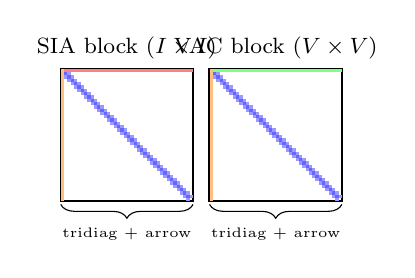
\begin{tikzpicture}[scale=0.042]
  % SIA block
  \draw[thick] (0,0) rectangle (40,40);
  \node[above] at (20,40) {\footnotesize SIA block ($I \times I$)};

  % Tridiagonal
  \foreach \i in {0,1,...,38} {
    \fill[blue!60] (\i, 39-\i) rectangle (\i+1, 40-\i);
    \fill[blue!40] (\i+1, 39-\i) rectangle (\i+2, 40-\i);
    \fill[blue!40] (\i, 38-\i) rectangle (\i+1, 39-\i);
  }
  % Dense row 1 (top)
  \foreach \i in {0,...,39} {
    \fill[red!50] (\i, 39) rectangle (\i+1, 40);
  }
  % Dense column 1 (left)
  \foreach \i in {0,...,39} {
    \fill[red!50] (0, \i) rectangle (1, \i+1);
  }

  % VAC block
  \draw[thick] (45,0) rectangle (85,40);
  \node[above] at (65,40) {\footnotesize VAC block ($V \times V$)};
  % Tridiagonal
  \foreach \i in {0,1,...,38} {
    \pgfmathsetmacro{\x}{int(45+\i)}
    \fill[blue!60] (\x, 39-\i) rectangle (\x+1, 40-\i);
    \fill[blue!40] (\x+1, 39-\i) rectangle (\x+2, 40-\i);
    \fill[blue!40] (\x, 38-\i) rectangle (\x+1, 39-\i);
  }
  % Dense row 1
  \foreach \i in {0,...,39} {
    \pgfmathsetmacro{\x}{int(45+\i)}
    \fill[green!50] (\x, 39) rectangle (\x+1, 40);
  }
  % Dense column 1
  \foreach \i in {0,...,39} {
    \fill[green!50] (45, \i) rectangle (46, \i+1);
  }

  % Off-diagonal: rank-1 columns
  % J_IV: column at c_v[1] in SIA eqs
  \foreach \i in {0,...,39} {
    \fill[orange!50] (45, \i) rectangle (46, \i+1);
  }
  % J_VI: column at c_i[1] in VAC eqs
  \foreach \i in {0,...,39} {
    \fill[orange!50] (0, \i) rectangle (1, \i+1);
  }

  % Labels
  \draw[decorate,decoration={brace,amplitude=5pt,mirror}] (0,-1) -- (40,-1)
    node[midway,below=5pt] {\tiny tridiag + arrow};
  \draw[decorate,decoration={brace,amplitude=5pt,mirror}] (45,-1) -- (85,-1)
    node[midway,below=5pt] {\tiny tridiag + arrow};
\end{tikzpicture}
\caption{Jacobian sparsity for monomer-only reactions ($\im = \vm = 1$).
Each diagonal block is an arrowhead matrix (tridiagonal + one dense row
and column). Off-diagonal blocks are rank-1. Total non-zeros: $O(\Neq)$.}
\label{fig:arrow}
\end{figure}

The arrowhead system can be solved in $O(\Neq)$ operations using the
Sherman--Morrison formula (rank-2 update of a tridiagonal
solve)~\cite{GolubVanLoan2013}.

%======================================================================
\section{Case~2: Coalescence ($\im > 1$, $\vm > 1$)}
\label{sec:coal}
%======================================================================

When multiple mobile species participate in coalescence
(e.g., $\im = 10$, $\vm = 5$), each SIA equation for cluster~$n$
acquires the following additional dependencies:

\begin{itemize}
  \item \textbf{Coalescence gain:}
    $\sum_{k=1}^{\min(n-1,\im)} \Kii_{k,n-k}\,c_{k}^{(i)}\,c_{n-k}^{(i)}$
    $\Rightarrow$ depends on $c_{n-k}^{(i)}$ for $k = 1,\ldots,\im$
    (band of width~$\im$ below the diagonal).

  \item \textbf{Coalescence loss:}
    $c_{n}^{(i)}\sum_{k=1}^{\im} \Kii_{n,k}\,c_{k}^{(i)}$
    $\Rightarrow$ depends on $c_{k}^{(i)}$ for $k = 1,\ldots,\im$
    ($\im$ dense columns).

  \item \textbf{V--I annihilation gain:}
    $\sum_{k=1}^{\vm} \Kvi_{k,n+k}\,c_{k}^{(v)}\,c_{n+k}^{(i)}$
    $\Rightarrow$ depends on $c_{n+k}^{(i)}$ for $k = 1,\ldots,\vm$
    (band of width~$\vm$ above the diagonal).

  \item \textbf{V--I annihilation loss:}
    $\sum_{k=1}^{\vm} \Kvi_{k,n}\,c_{k}^{(v)}\,c_{n}^{(i)}$
    $\Rightarrow$ depends on $c_{k}^{(v)}$ for $k = 1,\ldots,\vm$
    ($\vm$ dense columns in the off-diagonal block).
\end{itemize}

\subsection{Bordered-banded decomposition}

The full Jacobian admits the decomposition:
\begin{equation}
  \boxed{J = T + U\,W\,V^{T}}
  \label{eq:bordered_banded}
\end{equation}
where:
\begin{itemize}
  \item $T \in \RR^{\Neq \times \Neq}$ is \textbf{banded} with
    half-bandwidth
    \begin{equation}
      \bw = \max(2\im, \,2\vm) + 1,
      \label{eq:bandwidth}
    \end{equation}
    capturing emission (nearest-neighbor), local coalescence
    gain/loss (within the band), and diagonal terms
    (sinks, self-reaction).

  \item $U \in \RR^{\Neq \times \rank}$ collects the $\rank$ dense
    columns, where
    \begin{equation}
      \rank = \im + \vm.
      \label{eq:rank}
    \end{equation}
    These arise because each mobile species $c_{k}^{(i)}$
    ($k = 1,\ldots,\im$) and $c_{k}^{(v)}$ ($k = 1,\ldots,\vm$)
    appears in \emph{every} equation of the opposing (and same-species)
    block through coalescence loss and annihilation loss.

  \item $W \in \RR^{\rank \times \rank}$ is a small correction
    matrix, and $V \in \RR^{\Neq \times \rank}$ encodes the
    corresponding row structure.
\end{itemize}

\begin{figure}[H]
\centering
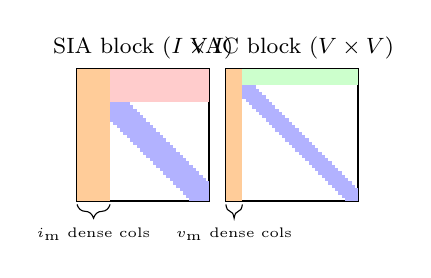
\begin{tikzpicture}[scale=0.042]
  % SIA block
  \draw[thick] (0,0) rectangle (40,40);
  \node[above] at (20,40) {\footnotesize SIA block ($I \times I$)};

  % Band (width ~10 on each side)
  \foreach \i in {0,...,39} {
    \foreach \j in {-5,...,5} {
      \pgfmathsetmacro{\col}{int(\i+\j)}
      \pgfmathsetmacro{\row}{int(39-\i)}
      \ifnum\col>-1
        \ifnum\col<40
          \fill[blue!30] (\col, \row) rectangle (\col+1, \row+1);
        \fi
      \fi
    }
  }

  % Dense columns 1..10 (mobile SIA)
  \foreach \c in {0,...,9} {
    \foreach \i in {0,...,39} {
      \fill[red!40] (\c, \i) rectangle (\c+1, \i+1);
    }
  }
  % Dense rows 1..10
  \foreach \c in {0,...,9} {
    \foreach \i in {0,...,39} {
      \fill[red!20] (\i, 39-\c) rectangle (\i+1, 40-\c);
    }
  }

  % VAC block
  \draw[thick] (45,0) rectangle (85,40);
  \node[above] at (65,40) {\footnotesize VAC block ($V \times V$)};

  % Band (width ~5)
  \foreach \i in {0,...,39} {
    \foreach \j in {-3,...,3} {
      \pgfmathsetmacro{\col}{int(45+\i+\j)}
      \pgfmathsetmacro{\row}{int(39-\i)}
      \ifnum\col>44
        \ifnum\col<85
          \fill[blue!30] (\col, \row) rectangle (\col+1, \row+1);
        \fi
      \fi
    }
  }

  % Dense columns 1..5 (mobile VAC)
  \foreach \c in {0,...,4} {
    \pgfmathsetmacro{\x}{int(45+\c)}
    \foreach \i in {0,...,39} {
      \fill[green!40] (\x, \i) rectangle (\x+1, \i+1);
    }
  }
  % Dense rows 1..5
  \foreach \c in {0,...,4} {
    \foreach \i in {0,...,39} {
      \pgfmathsetmacro{\x}{int(45+\i)}
      \fill[green!20] (\x, 39-\c) rectangle (\x+1, 40-\c);
    }
  }

  % Off-diagonal coupling columns
  % J_IV: v_mobile dense columns in SIA block rows
  \foreach \c in {0,...,4} {
    \pgfmathsetmacro{\x}{int(45+\c)}
    \foreach \i in {0,...,39} {
      \fill[orange!40] (\x, \i) rectangle (\x+1, \i+1);
    }
  }
  % J_VI: i_mobile dense columns in VAC block rows
  \foreach \c in {0,...,9} {
    \foreach \i in {0,...,39} {
      \fill[orange!40] (\c, \i) rectangle (\c+1, \i+1);
    }
  }

  % Labels
  \draw[decorate,decoration={brace,amplitude=5pt,mirror}] (0,-1) -- (10,-1)
    node[midway,below=5pt] {\tiny $\im$ dense cols};
  \draw[decorate,decoration={brace,amplitude=5pt,mirror}] (45,-1) -- (50,-1)
    node[midway,below=5pt] {\tiny $\vm$ dense cols};
\end{tikzpicture}
\caption{Jacobian sparsity for coalescence
($\im = 10$, $\vm = 5$).
Each diagonal block is banded (blue) with $\im$ or $\vm$ dense
columns (red/green) from mobile species.
Off-diagonal blocks (orange) have the same rank-$\im$ or rank-$\vm$ structure.}
\label{fig:bordered}
\end{figure}

\subsection{Consistency with the monomer case}

Setting $\im = \vm = 1$ in \eqref{eq:bordered_banded} recovers the
arrowhead structure of Section~\ref{sec:monomer}: the band reduces to
a tridiagonal ($\bw = 3$) and the border is rank-2 ($\rank = 2$).
The Woodbury preconditioner described in Section~\ref{sec:woodbury}
thus handles both cases with a \emph{single code path}---no
special-casing is needed.

%======================================================================
\section{Limitations of GMRES for Bordered-Banded Systems}
\label{sec:gmres}
%======================================================================

CVODE's BDF method requires solving the Newton correction system
\begin{equation}
  (I - \gamma\,J)\,\Delta\mathbf{y} = -\mathbf{g}
  \label{eq:newton}
\end{equation}
at each time step, where $\gamma = h\beta$ involves the step size~$h$
and the BDF coefficient~$\beta$. The matrix $M = I - \gamma J$ inherits
the bordered-banded structure of~$J$.

\subsection{Dense direct solver}

The default dense LU factorization costs $O(\Neq^{3})$ per Newton
step. For $\Neq = I + V + 2 \approx 20{,}000$, this is
$\sim 8 \times 10^{12}$ floating-point operations per step---entirely
impractical for production runs.

\subsection{Unpreconditioned GMRES}

GMRES~\cite{SaadSchultz1986} is an iterative Krylov method that
computes
$\Delta\mathbf{y} \approx \arg\min_{\mathbf{x} \in \mathcal{K}_{k}}
\|M\mathbf{x} - \mathbf{b}\|_{2}$
over the Krylov subspace $\mathcal{K}_{k}(M,\mathbf{b})$.
Each iteration costs $O(\Neq)$ (one matrix--vector product plus
Gram--Schmidt), but the number of iterations depends on the
\emph{condition number} $\kappa(M)$.

For the bordered-banded Jacobian, the eigenvalue spectrum is
problematic:
\begin{enumerate}
  \item The dense columns from mobile species couple all $\Neq$
    equations, creating $O(\rank)$ eigenvalues that are well separated
    from the banded spectrum of~$T$.
  \item The stiffness ratio between fast monomer reactions and slow
    large-cluster evolution spans 10--15 orders of magnitude,
    producing $\kappa(M) \sim 10^{10}$--$10^{15}$.
  \item GMRES convergence stalls when the eigenvalue distribution has
    widely separated outliers~\cite{Saad2003}, which is exactly the
    pattern created by the low-rank border.
\end{enumerate}

In practice, unpreconditioned GMRES requires $O(\Neq)$ iterations
(i.e., the full Krylov subspace), negating its advantage over a direct
solver.

\subsection{Diagonal (Jacobi) preconditioner}

The current RadCluster implementation offers a Jacobi (diagonal)
preconditioner:
\begin{equation}
  P_{\rm Jacobi} = \diag(M) = \diag(1 - \gamma\,J_{kk}).
  \label{eq:jacobi}
\end{equation}
This captures only the self-reaction rates (sinks, self-coalescence)
and completely misses:
\begin{itemize}
  \item The \textbf{banded coupling} from emission and local
    coalescence ($\sim 2\bw$ off-diagonal entries per row).
  \item The \textbf{dense-column coupling} from mobile species
    appearing in every equation ($\rank$ dense columns).
  \item The \textbf{cross-species coupling} between SIA and VAC
    blocks.
\end{itemize}

For the coalescence case, the Jacobi preconditioner reduces GMRES
iteration counts only modestly (from $O(\Neq)$ to perhaps
$O(\Neq/2)$), which is still far too many for efficiency.

%======================================================================
\section{Woodbury Preconditioner}
\label{sec:woodbury}
%======================================================================

\subsection{The Sherman--Morrison--Woodbury identity}

For any invertible $T$ and conformable $U, W, V$, the
Sherman--Morrison--Woodbury (SMW) identity~\cite{Woodbury1950,
Hager1989} states:
\begin{equation}
  \boxed{(T + U\,W\,V^{T})^{-1} =
  T^{-1} - T^{-1}\,U\,
  \bigl(W^{-1} + V^{T}\,T^{-1}\,U\bigr)^{-1}\,
  V^{T}\,T^{-1}}
  \label{eq:smw}
\end{equation}

Applied to $M = I - \gamma J = (I - \gamma T)
- \gamma\,U\,W\,V^{T}$, we define:
\begin{align}
  \hat{T} &= I - \gamma\,T \quad (\text{banded, bandwidth } \bw),
  \label{eq:That} \\
  \hat{U} &= \gamma\,U, \quad \hat{V} = V,
  \label{eq:UVhat}
\end{align}
so that $M = \hat{T} - \hat{U}\,W\,\hat{V}^{T}$ and
\begin{equation}
  M^{-1} = \hat{T}^{-1}
  + \hat{T}^{-1}\,\hat{U}\,
  \bigl(W^{-1} - \hat{V}^{T}\,\hat{T}^{-1}\,\hat{U}\bigr)^{-1}\,
  \hat{V}^{T}\,\hat{T}^{-1}.
  \label{eq:prec}
\end{equation}

\subsection{Construction of $T$, $U$, $V$, $W$}

The decomposition $J = T + U\,W\,V^{T}$ is constructed as follows:

\begin{enumerate}
  \item \textbf{Band extraction:} $T$ is the restriction of $J$ to
    entries within bandwidth~$\bw$ of the diagonal. This captures
    emission, local coalescence, sinks, and all
    nearest-neighbor coupling. Since $J$ is not available
    analytically, we approximate $T$ by \emph{banded finite
    differences}: perturbing groups of state variables that are
    more than~$\bw$ apart (Curtis--Powell--Reid
    coloring~\cite{CurtisPowellReid1974}), requiring only
    $2\bw + 1$ RHS evaluations instead of~$\Neq$.

  \item \textbf{Dense columns:} $U$ collects the $\rank = \im + \vm$
    dense columns of $J$ corresponding to mobile species indices.
    Column~$j$ of~$U$ is approximated by a single finite-difference
    perturbation of $y_{j}$, minus the entries already captured
    in~$T$ (to avoid double-counting).

  \item \textbf{Row structure:} For the preconditioner we use the
    simplification $W = I_{\rank}$ and let $V^{T}$ encode the dense
    rows. In practice, the dense rows correspond to the same mobile
    species indices as the dense columns, giving $V = U$ to leading
    order (the Jacobian sub-blocks involving mobile species are
    approximately symmetric in their sparsity pattern, though not in
    their values).

  \item \textbf{Simplification:} When the dense column/row indices
    coincide (as they do here), the border can be represented as:
    \begin{equation}
      J \approx T + \sum_{j=1}^{\rank}
      (\mathbf{J}_{\cdot,j} - \mathbf{T}_{\cdot,j})\,\mathbf{e}_{j}^{T},
    \end{equation}
    where $\mathbf{J}_{\cdot,j}$ is the $j$-th column of $J$
    (obtained by a single finite-difference probe) and
    $\mathbf{T}_{\cdot,j}$ is its banded restriction. This is a
    rank-$\rank$ correction with
    $U = [\mathbf{J}_{\cdot,1} - \mathbf{T}_{\cdot,1},\ldots,
    \mathbf{J}_{\cdot,\rank} - \mathbf{T}_{\cdot,\rank}]$,
    $W = I$, $V = [\mathbf{e}_{1},\ldots,\mathbf{e}_{\rank}]$.
\end{enumerate}

\subsection{Algorithm}

\begin{algorithm}[H]
\caption{Woodbury preconditioner setup}
\label{alg:setup}
\begin{algorithmic}[1]
  \Require State $\mathbf{y}$, RHS function $\mathbf{f}$, BDF
    parameter $\gamma$
  \State Evaluate base RHS: $\mathbf{f}_{0} \gets \mathbf{f}(\mathbf{y})$
  \State \textbf{// Band extraction via CPR coloring}
  \For{color $c = 1,\ldots,2\bw+1$}
    \State Perturb: $\tilde{\mathbf{y}} \gets \mathbf{y}$;
      $\tilde{y}_{j} \gets y_{j} + \delta_{j}$ for all $j$ with
      $j \bmod (2\bw+1) = c$
    \State $\tilde{\mathbf{f}} \gets \mathbf{f}(\tilde{\mathbf{y}})$
    \For{each perturbed index $j$}
      \State $T_{k,j} \gets (\tilde{f}_{k} - f_{0,k})/\delta_{j}$
        for $|k - j| \le \bw$
    \EndFor
  \EndFor
  \State \textbf{// Dense column probes for mobile species}
  \For{$j \in \{\text{mobile SIA indices}\} \cup \{\text{mobile VAC indices}\}$}
    \State $\tilde{\mathbf{y}} \gets \mathbf{y}$;
      $\tilde{y}_{j} \gets y_{j} + \delta_{j}$
    \State $\mathbf{u}_{j} \gets (\mathbf{f}(\tilde{\mathbf{y}}) - \mathbf{f}_{0})/\delta_{j}
      - T_{\cdot,j}$
    \Comment{Subtract banded part}
  \EndFor
  \State \textbf{// Form preconditioner matrices}
  \State $\hat{T} \gets I - \gamma\,T$
  \State Factor $\hat{T}$ via banded LU (LAPACK \texttt{dgbtrf})
  \State Solve $\hat{T}^{-1}\hat{U}$ via $\rank$ banded back-solves
  \State Form $S \gets I_{\rank} + \gamma\,V^{T}\,\hat{T}^{-1}\hat{U}$
    \Comment{$\rank \times \rank$ Schur complement}
  \State Factor $S$ via dense LU (LAPACK \texttt{dgetrf})
\end{algorithmic}
\end{algorithm}

\begin{algorithm}[H]
\caption{Woodbury preconditioner solve: $P^{-1}\mathbf{r} = \mathbf{z}$}
\label{alg:solve}
\begin{algorithmic}[1]
  \Require Residual $\mathbf{r}$, factored $\hat{T}$, factored $S$,
    pre-computed $\hat{T}^{-1}\hat{U}$
  \State $\mathbf{w}_{1} \gets \hat{T}^{-1}\mathbf{r}$
    \Comment{Banded back-solve, $O(\Neq\,\bw)$}
  \State $\mathbf{w}_{2} \gets V^{T}\,\mathbf{w}_{1}$
    \Comment{Extract $\rank$ components, $O(\rank)$}
  \State $\mathbf{w}_{3} \gets S^{-1}\,\mathbf{w}_{2}$
    \Comment{Dense solve, $O(\rank^{2})$}
  \State $\mathbf{z} \gets \mathbf{w}_{1}
    - (\hat{T}^{-1}\hat{U})\,\mathbf{w}_{3}$
    \Comment{$O(\Neq\,\rank)$}
\end{algorithmic}
\end{algorithm}

\subsection{Computational cost}

\begin{table}[H]
\centering
\caption{Operation counts per Newton step. $\Neq \approx 20{,}000$,
$\bw = 21$, $\rank = 15$ (for $\im = 10$, $\vm = 5$).}
\label{tab:cost}
\begin{tabular}{@{}lcccc@{}}
\toprule
\textbf{Method} & \textbf{Setup} & \textbf{Solve} &
  \textbf{RHS evals} & \textbf{GMRES iters} \\
\midrule
Dense direct & $O(\Neq^{3})$ & $O(\Neq^{2})$ & $\Neq$ & --- \\
 & $\sim 8 \times 10^{12}$ & $\sim 4 \times 10^{8}$ & 20{,}000 & \\
\addlinespace
Jacobi + GMRES & $O(\Neq)$ & $O(\Neq\,k)$ & 1 & $k \gg 1$ \\
 & $\sim 2 \times 10^{4}$ & --- & & $\sim$1000+ \\
\addlinespace
\textbf{Woodbury + GMRES} & $O(\Neq\,\bw^{2})$ & $O(\Neq\,\bw)$ &
  $2\bw + 1 + \rank$ & 1--3 \\
 & $\sim 9 \times 10^{6}$ & $\sim 4 \times 10^{5}$ & 58 & \\
\bottomrule
\end{tabular}
\end{table}

The Woodbury preconditioner achieves a \textbf{speedup of
$\sim\!10^{5}$} over the dense solver and requires only
$2\bw + 1 + \rank = 58$ RHS evaluations for setup (vs.\ $\Neq =
20{,}000$ for a full finite-difference Jacobian).

\subsection{Monomer-case reduction}

For $\im = \vm = 1$: $\bw = 3$ (tridiagonal), $\rank = 2$.
\begin{itemize}
  \item Setup: $O(\Neq \cdot 9 + 8) = O(\Neq)$
    --- effectively a tridiagonal LU plus a $2 \times 2$ Schur
    complement.
  \item Solve: $O(\Neq \cdot 3 + 2) = O(\Neq)$
    --- one tridiagonal back-solve plus a $2 \times 2$ dense solve.
  \item RHS evaluations for probing: $2 \cdot 3 + 1 + 2 = 9$.
\end{itemize}
This is the \emph{optimal} solver for arrowhead
matrices~\cite{GolubVanLoan2013}, confirming that the Woodbury
preconditioner does not degrade performance in the monomer limit.

%======================================================================
\section{Perturbation Size for Finite Differences}
\label{sec:perturbation}
%======================================================================

The perturbation for column~$j$ of the Jacobian is chosen as
\begin{equation}
  \delta_{j} = \sqrt{u_{\rm round}} \cdot \max(|y_{j}|, \, y_{\rm typ})
  \cdot \operatorname{sign}(y_{j}),
  \label{eq:delta}
\end{equation}
where $u_{\rm round} \approx 10^{-16}$ is machine epsilon and
$y_{\rm typ}$ is a typical concentration scale (set to the absolute
tolerance). This is the same formula used internally by CVODE for its
difference-quotient Jacobian~\cite{HindmarshEtAl2005}.

%======================================================================
\section{Summary}
\label{sec:summary}
%======================================================================

\begin{enumerate}
  \item The RadCluster Jacobian has a \textbf{bordered-banded}
    structure: banded (bandwidth $\bw \sim 2\max(\im, \vm)$) plus
    a low-rank dense border (rank $\rank = \im + \vm$) from
    mobile species coupling.

  \item The \textbf{monomer case} ($\im = \vm = 1$) is a special
    case: the Jacobian reduces to an \textbf{arrowhead} matrix
    (tridiagonal + rank-2 border).

  \item \textbf{Dense direct} solvers cost $O(\Neq^{3})$ and are
    impractical for $\Neq > 1000$.

  \item \textbf{Unpreconditioned GMRES} fails because the
    bordered-banded eigenvalue spectrum has widely separated
    outliers from the dense border.

  \item The \textbf{Jacobi preconditioner} captures only diagonal
    entries, missing the dominant banded and dense-column coupling.

  \item The \textbf{Woodbury preconditioner} exploits the
    bordered-banded decomposition via the SMW identity:
    \begin{itemize}
      \item Setup: banded LU ($O(\Neq\,\bw^{2})$) +
        $\rank \times \rank$ Schur complement ($O(\rank^{3})$).
      \item Solve: banded back-solve ($O(\Neq\,\bw)$) +
        Woodbury correction ($O(\Neq\,\rank)$).
      \item GMRES converges in 1--3 iterations.
      \item Speedup $\sim 10^{5}$ over dense direct.
      \item Subsumes the arrowhead case with no code changes.
    \end{itemize}
\end{enumerate}

%======================================================================
\bibliographystyle{plainnat}
\begin{thebibliography}{10}

\bibitem[Curtis et~al.(1974)]{CurtisPowellReid1974}
A.~R. Curtis, M.~J.~D. Powell, and J.~K. Reid.
\newblock On the estimation of sparse {J}acobian matrices.
\newblock \emph{IMA J.\ Appl.\ Math.}, 13(1):117--119, 1974.

\bibitem[Ghoniem(2026)]{Ghoniem2026}
N.~M. Ghoniem.
\newblock A cluster dynamics model for radiation damage evolution in
  ferritic-martensitic steels.
\newblock Technical report, UCLA, 2026.
\newblock RadCluster formulation document.

\bibitem[Golub and Van~Loan(2013)]{GolubVanLoan2013}
G.~H. Golub and C.~F. Van~Loan.
\newblock \emph{Matrix Computations}.
\newblock Johns Hopkins University Press, 4th edition, 2013.

\bibitem[Hager(1989)]{Hager1989}
W.~W. Hager.
\newblock Updating the inverse of a matrix.
\newblock \emph{SIAM Review}, 31(2):221--239, 1989.

\bibitem[Hindmarsh et~al.(2005)]{HindmarshEtAl2005}
A.~C. Hindmarsh, P.~N. Brown, K.~E. Grant, S.~L. Lee, R.~Serban,
  D.~E. Shumaker, and C.~S. Woodward.
\newblock {SUNDIALS}: Suite of nonlinear and differential/algebraic equation
  solvers.
\newblock \emph{ACM Trans.\ Math.\ Software}, 31(3):363--396, 2005.

\bibitem[Saad(2003)]{Saad2003}
Y.~Saad.
\newblock \emph{Iterative Methods for Sparse Linear Systems}.
\newblock SIAM, 2nd edition, 2003.

\bibitem[Saad and Schultz(1986)]{SaadSchultz1986}
Y.~Saad and M.~H. Schultz.
\newblock {GMRES}: A generalized minimal residual algorithm for solving
  nonsymmetric linear systems.
\newblock \emph{SIAM J.\ Sci.\ Stat.\ Comput.}, 7(3):856--869, 1986.

\bibitem[Woodbury(1950)]{Woodbury1950}
M.~A. Woodbury.
\newblock Inverting modified matrices.
\newblock Technical Report~42, Statistical Research Group, Princeton
  University, 1950.

\end{thebibliography}

\end{document}
